\section{Λειτουργικά Συστήματα}

\lstset{language=C++}

\subsection{Παράλληλες διεργασίες}

\subsubsection{Γράφος προτεραιότητας – εντολές παραλληλισμού}

\begin{figure}[!ht]
	\centering
	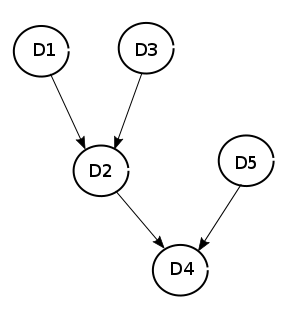
\includegraphics[width=0.4\textwidth]{grafos.png}
	\caption{Παράδειγμα Γράφου προτεραιότητας}
\end{figure}

\begin{lstlisting}[caption={Εντολές παραλληλισμού του παραπάνω παραδείγματος}]
cobegin
	begin
		cobegin
		D1;
		D3;
		coend;
		D2;
	end;
	D5;
coend;
D4;
\end{lstlisting}

\subsubsection{Συγχρονισμός} 


\paragraph{Κρίσιμες περιοχές - Αμοιβαίος αποκλεισμός}

\begin{itemize}
	\item 	Κρίσιμη περιοχή: Η περιοχή που περιέχει προσπελάσεις σε
		διαμοιραζόμενες περιοχές μνήμης ή αρχεία
	\item	Επιθυμητός ο αμοιβαίος αποκλεισμός: αποκλεισμός μιας
		διεργασίας από κάποια ενέργεια που ταυτόχρονα επιτελεί
		κάποια άλλη διεργασία
	\item	Λύση: Συγχρονισμός που προϋποθέτει τις ακόλουθες
		συνθήκες:
		\begin{enumerate}
			\item	Δυο διεργασίες δεν βρίσκονται ποτέ ταυτόχρονα στα κρίσιμα τμήματά
				τους (αμοιβαίος αποκλεισμός).
			\item	Δεν επιτρέπονται υποθέσεις σε ό,τι αφορά την ταχύτητα ή το πλήθος
				των επεξεργαστών.
			\item	Διεργασία που δεν βρίσκεται σε κρίσιμο τμήμα δεν επιτρέπεται να
				αναστείλει άλλες διεργασίες (progress).
			\item	Δεν επιτρέπεται η επ’ αόριστον αναμονή μιας διεργασίας για να
				εισέλθει στο κρίσιμο τμήμα της (bounded waiting).
		\end{enumerate}
\end{itemize}

\paragraph{Κρίσιμη περιοχή - Υλοποίηση}

\indent Πως μπορεί να υλοποιηθεί μια κρίσιμη περιοχή;
με «έξυπνες» λύσεις που βασίζονται στο λογισμικό
με τη χρήση «εργαλείων» που προσφέρουν τα ΛΣ
(αλλά και κάποιες – παλαιότερες - υψηλές γλώσσες
προγραμματισμού) όπως είναι οι σημαφόροι και οι
κρίσιμες περιοχές / κρίσιμες περιοχές υπό συνθήκη
με τη χρήση των δυνατοτήτων του hardware (π.χ. η
συνάρτηση TestAndSet)

\subsubsection{Mutex - Peterson}

Οι interested0,1 εκφράζουν πρόθεση να μπουν στην κρίσιμη περιοχή, 
ενώ η turn δηλώνει ποιος έχει σειρά να μπει.


\begin{lstlisting}[caption=Init Values]
turn = 0;
interested0 = false;
interested1 = false;
\end{lstlisting}

\begin{lstlisting}[caption=Process P0]
while(true){
	interested0 = true;
	turn = 0;
	while(interested1==true && turn == 0){}
	critical_section();
	interested0 = false;
	non_critical_section();
}
\end{lstlisting}

\begin{lstlisting}[caption=Process P1]
while(true){
	interested1 = true;
	turn = 1;
	while(interested0==true && turn == 1){}
	critical_section():
	interested1 = false;
	non_critical_section();
}
\end{lstlisting}

\subsubsection{Mutex - Dekker}

Αν και οι δύο διεργασίες θέλουν να
εισέλθουν στην κρίσιμη περιοχή, θα
θέσουν τις αντίστοιχες μεταβλητές true.
Η μεταβλητή turn θα λειτουργήσει τότε ως
διαιτητής για να αποτρέψει τη λιμοκτονία
(starvation) δηλαδή το να μη μπορεί καμία
διεργασία να μπει στην κρίσιμη περιοχή.

\begin{lstlisting}[caption=Init values]
turn = 1;
interested0 = false;
interested1 = false;
\end{lstlisting}

\begin{lstlisting}[caption=Process P0]
while(true){
	interested0 = true;
	while(interested1==true){
		if(turn==1){
			interested0 = false;
			while(turn==1){}
			interested0 = true;
		}
	}
	critical_section():
	turn = 1;
	interested0 = false;
	non_critical_section;
}
\end{lstlisting}

\begin{lstlisting}[caption=Process P1]
while(true){
	interested1 = true;
	while(interested0==true){
		if(turn==0){
			interested1 = false;
			while(turn==0){}
			interested1 = true;
		}
	}
	critical_section();
	turn = 0;
	interested1 = false;
	non_critical_section();
}
\end{lstlisting}

\subsection{Σημαφόροι}

\begin{lstlisting}[caption=wait or P or down function implementaion]
void signal(int *s){
	while(*s<=0) {}
	*s = *s - 1;
}
\end{lstlisting}

\begin{lstlisting}[caption=signal or V or up function implementaiton]
void wait(int *s){
	*s = *s + 1;
}
\end{lstlisting}

\begin{lstlisting}[caption=General semaphore implementation]
void wait(semaphore *u){
	u->count--;
	if(u->count < 0){
		*u.queue.push(this_process);
		this_process.block();
	}
}

void signal(semaphore *u){
	u->count++
	if(u->count<=0){
		*u.queue.pop();
		*u.ready_queue.push(this_process);
	}
}
\end{lstlisting}

Κάθε σημαφόρος διαθέτει μια ουρά στην οποία συνδέονται οι διεργασίες που
έχουν ανασταλεί λόγω της εκτέλεσης ενός wait (συχνά αναφερόμαστε σε αυτές
ως «μπλοκαρισμένες διεργασίες»).

\subsubsection{Ορισμός σημαφόρου}

\begin{itemize}
	\item	Υψηλότερου επιπέδου δομή για να πετύχουμε αμοιβαίο αποκλεισμό
	\item	Μέσω δύο πράξεων
		\begin{itemize}
			\item	Wait (S) ή P(S) ή Down(S)
			\item	Signal (S) ή V(S) ή Up(S)
		\end{itemize}
	\item	Μια εντολή σημαφόρου (wait ή signal) με ευθύνη
		του ΛΣ εκτελείται ατομικά, δηλ. αν μια διεργασία
		αρχίσει να εκτελεί π.χ. ένα wait σε ένα σημαφόρο,
		δεν επιτρέπεται να διακοπεί και η εκτέλεσή του
		wait αντιμετωπίζεται ως ένα αδιαίρετο βήμα.
\end{itemize}

\subsubsection{Είδη σημαφόρων}

\begin{itemize}
	\item	Βinary
		\begin{itemize}
			\item	Παίρνει τιμές 0 και 1
			\item	Προστατεύει την προσπέλαση των κρίσιμων περιοχών
			\item	mutex
		\end{itemize}
	\item	Γενική σημαφόρος
		\begin{itemize}
			\item	Μπορεί να παίρνει οποιαδήποτε θετική τιμή
		\end{itemize}
\end{itemize}

\textbf{Προσοχή:} Όλοι οι σημαφόροι πρέπει να είναι αρχικοποιημένοι!!!

\subsubsection{Προστασία κρίσιμων περιοχών}

Έστω δύο διεργασίες Α και Β που ενεργούν
πάνω στο υπόλοιπο Χ ενός λογαριασμού τράπεζας:

\begin{lstlisting}
semaphore mutex = 1; // mutex init value

void process_a(){
	wait (mutex);
	X = X + amount;
	signal (mutex);
}

void process_b(){
	wait (mutex);
	X = X - amount;
	signal (mutex);
}
\end{lstlisting}

\subsubsection{Συγχρονισμός διεργασιών}

Έστω δύο διεργασίες Α και Β. H A τυπώνει τη
λέξη ping και η Β τη λέξη pong:

\begin{lstlisting}
semaphore sem_a = 1;
semaphore sem_b = 0;

void process_a(){
	wait(sem_a);
	print("ping");
	signal(sem_b);
}

void process_b(){
	wait(sem_b);
	print("pong");
	signal(sem_a);
}
\end{lstlisting}

\subsubsection{Αναγνώστες και Συγγραφείς}

\begin{lstlisting}
semaphore rc_sem, write_sem = 1;
int readcount = 0;

void reader(){
	wait(rc_sem);
	readcount++;
	if(readcount = 1)
		wait(write_sem);
	signal(rc_sem);
	
	read(myfile, 'r');
	
	wait(rc_sem);
	readcount--;
	if(readcount = 0)
		signal(write_sem);
	signal(rc_sem);
}

void writer(){
	wait(write_sem);
	write(myfile, 'w');
	signal(write_sem);
}
\end{lstlisting}


\subsubsection{Χρονοδρομολόγηση διεργασιών}

\begin{itemize}
	\item	\textbf{Μη - Προεκχωρητικοί αλγόριθμοι:}
		Επιτρέπουν στις επιλεγμένες διεργασίες να κρατήσουν την
		ΚΜΕ μέχρι να ανασταλεί ή να τερματίσει.
	\item	\textbf{Προεκχωρητικοί αλγόριθμοι:}
		Η εκτέλεση της διεργασίας που κατέχει την ΚΜΕ
		διακόπτεται περιοδικά και ο χρονοδρομολογητής καλείται
		να αποφασίσει ποια θα είναι η επόμενη.
	\item	Μετρικές απόδοσης
		\begin{itemize}
			\item 	Χρόνος διεκπεραίωσης: $ \text{ΧΔ} = t_\text{περάτωσης εκτέλεσης} - t_\text{εισόδου στο σύστημα} $
			\item 	Χρόνος Αναμονής: $ \text{ΧΑ} = \text{ΧΔ} - t_\text{χρόνος εκτέλεσης εργασίας στην ΚΜΕ} $
			\item 	$ \text{Ρυθμός απόδοσης} = \frac{\text{Αρ. διεργ. που ολοκληρώνονται}}{t} $
			\item	$ \text{Χρόνος απόκρισης} = t_\text{έναρξης εξυπηρέτησης} – t_\text{υποβολής} $
		\end{itemize}
\end{itemize}

\paragraph{Αλγόριθμοι Χρονοδρομολόγησης}

\begin{itemize}
	\item	First Come First Served - FCFS
		\begin{itemize}
			\item	Δίκαιος Αλγόριθμος.
			\item	Παρουσιάζει πρόβλημα αν μια μεγάλη διεργασία μπει πριν από μια ή περισσότερες
				μικρές διεργασίες.
		\end{itemize}
	\item	Round Robin - RR (προεκχωρητική έκδοση FCFS)
		\begin{itemize}
			\item	Εξαιρετικά δίκαιος αλγόριθμός.
			\item	Δεν προκαλεί καθυστερήσεις στις μικρές διεργασίες, γεγονός που τον κάνει ιδανικό
				για συστήματα διαμοιρασμού χρόνου.
			\item	Αν το κβάντο χρόνου είναι µεγάλο, µπορεί να προκληθούν µεγάλοι χρόνοι
				απόκρισης σε µικρές αλληλεπιδραστικές διεργασίες.
			\item	Αν το κβάντο χρόνου είναι µικρό, εναλλαγές διεργασιών γίνονται πολύ συχνά, 
				γεγονός που µειώνει την αποδοτικότητα της ΚΜΕ.
		\end{itemize}
	\item	Shortest Job First - SJF
		\begin{itemize}
			\item	Όπως και ο αλγόριθμος προτεραιοτήτων μπορεί να προκαλέσει παρατεταμένη
				στέρηση για μεγάλες διεργασίες.
			\item	Πολύ δύσκολος στην υλοποίηση γιατί δεν γνωρίζουμε εκ των προτέρων πόσο
				χρόνο θα χρειαστεί η κάθε διεργασία.
		\end{itemize}
	\item 	Shortest Remaining Time First – SRTF (προεκχωρητική έκδοση SJF)
	\item	Priority
		\begin{itemize}
			\item	Δρομολόγηση διεργασιών βάση προτεραιοτήτων
			\item	Μπορεί να οδηγήσει σε παρατεταµένη στέρηση αν στο σύστηµα εισέρχονται διαρκώς
				διεργασίες µε µεγαλύτερες προτεραιότητες από εκείνη κάποιας άλλης διεργασίας.
		\end{itemize}
\end{itemize}

\subsection{Μνήμη}

\subsubsection{Σελίδοποίηση}

\begin{figure}[!ht]
	\centering
	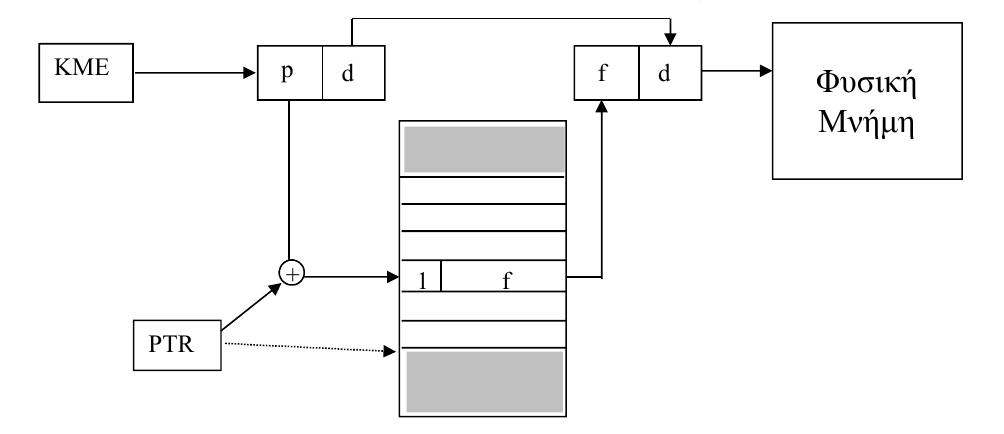
\includegraphics[width=0.5\textwidth]{paging.png}
	\caption{Paging}
\end{figure}

\begin{center}
\begin{tabularx}{0.5\textwidth}{|X|X|}
	\hline
	Όρος & Περιγραφή \\
	\hline
	p & Αριθμός σελίδας \\
	\hline
	f & Αριθμός Πλαισίου \\
	\hline
	d & Μετατόπιση (offset)\\
	\hline
	1 & Present bit (αν βρίσκεται η σελίδα στην μνήμη ή όχι) \\
	\hline
	ptr & {Page table register περιέχει τη διεύθυνση της φυσικής
	μνήμης όπου αρχίζει (έχει φορτωθεί) ο πίνακας σελίδων
	για την τρέχουσα διεργασία/πρόγραμμα } \\
	\hline
\end{tabularx}
\end{center}

\textbf{Προσοχή} Το + εδώ σημαίνει συνένωση όχι πρόσθεση!!! \\

\paragraph{Μορφή ιδεατής διεύθυνσης `U' (n bits):} Αριθμός Ιδεατής Σελίδας `p' (n-k bits) +
Μετατόπιση `d' (k bits) \\

\paragraph{Μετατροπή σε φυσική διεύθυνση Φ (σύνολο m bits):} Αριθμός φυσικής σελίδας `f' (m-k bits)  +
Μετατόπιση `d' (k bits)

\subsubsection{Μέσος Χρόνος Προσπέλασης Μνήμης}

Έστω ότι x (χρόνος προσπέλασης στους συσχετιστικούς καταχωρητές), y (χρόνος προσπέλασης της μνήμης),
p (ποσοστό επιτυχίας), p' ποσοστό αποτυχίας και $ 0 \le p, p' \le 1$, $ p + p' = 1$.

Για να υπολογίσουμε τον μέσο χρόνο προσπέλασης μνήμης (effective memory access time) κάνουμε:
$$ \text{Effective access time} = p \cdot (x+y) + p' \cdot (x+2y) $$

\subsubsection{Τμηματοποίηση}

\begin{figure}[!ht]
	\centering
	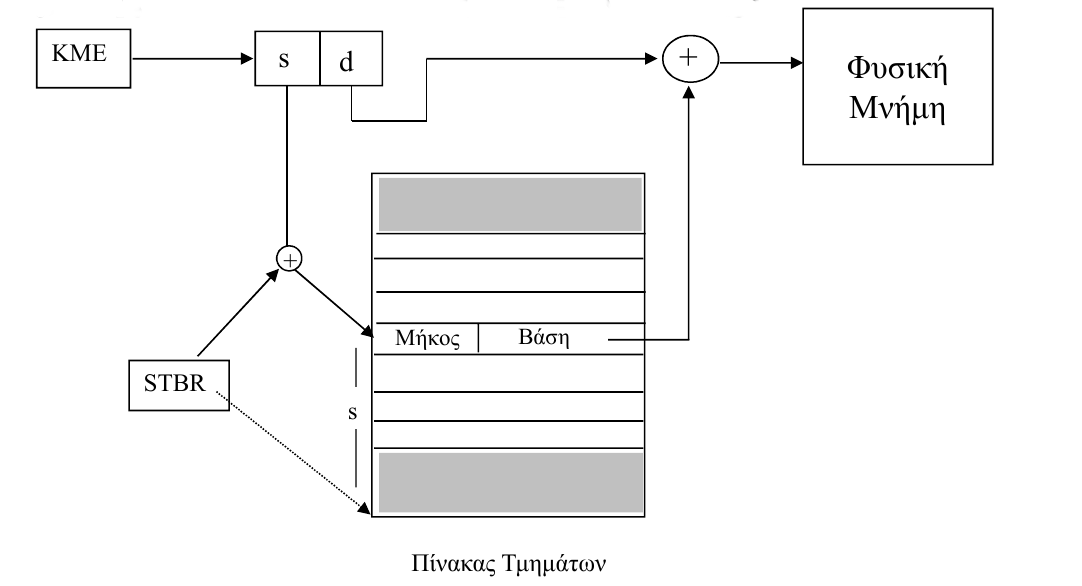
\includegraphics[width=0.5\textwidth]{segmentaion.png}
	\caption{segmentation}
\end{figure}

\begin{center}
\begin{tabularx}{0.5\textwidth}{|X|X|}
	\hline
	Όρος & Περιγραφή \\
	\hline
	s & Θέση στον πίνακα τμημάτων της διεργασίας \\
	\hline
	d & Μετατόπιση (offset). \textbf{Προσοχή} πρέπει να είναι μικρότερη από το μήκος. \\
	\hline
	STBR & {Segment Table Base Register: Σε ποια διεύθυνση
	της μνήμης αρχίζει ο πίνακας τμημάτων της διεργασίας μας} \\
	\hline
\end{tabularx}
\end{center}

\paragraph{Κάθε λογική διεύθυνση U (n bits) είναι στη μορφή:}
$$ \text{Αριθμός Λογικού Τμήματος }s (n-k~bits) + \text{ Μετατόπιση } d (k~bits) $$
$$ \text{Μέγιστος αριθμός τμημάτων: } 2^{n-k}\text{  Μέγιστο μέγεθος τμήματος: } 2^k $$
\paragraph{Μετατρέπεται σε μία Φυσική Διεύθυνση Φ στη μορφή:}
$$ \text{Διεύθυνση Βάσης Τμήματος } + \text{ Μετατόπιση } d (k~bits) $$

\subsubsection{Σελιδοποιημένη Τμηματοποίηση}

\paragraph{Η λογική διεύθυνση U (n bits) τώρα χωρίζεται σε 3 τμήματα.}
\begin{center}
\begin{tabularx}{0.95\textwidth}{|X|X|X|}
\hline
Αριθμός Τμήματος s(n-k bits) & \multicolumn{2}{|l|}{ + Μετατόπιση d (k bits)} \\
\hline
{} & Αρ. Σελίδας p & Μετατ. Σελίδας d' \\
\hline
\end{tabularx}
\end{center}

\paragraph{Και μετατρέπεται σε φυσική διεύθυνση Φ στη μορφή:}
\begin{center}
\begin{tabularx}{0.95\textwidth}{X X}
Αριθμός Φυσικής Σελίδας f(m-k' bits) & + Μετατόπιση d'(k' bits)
\end{tabularx}
\end{center}

\begin{figure}[!ht]
	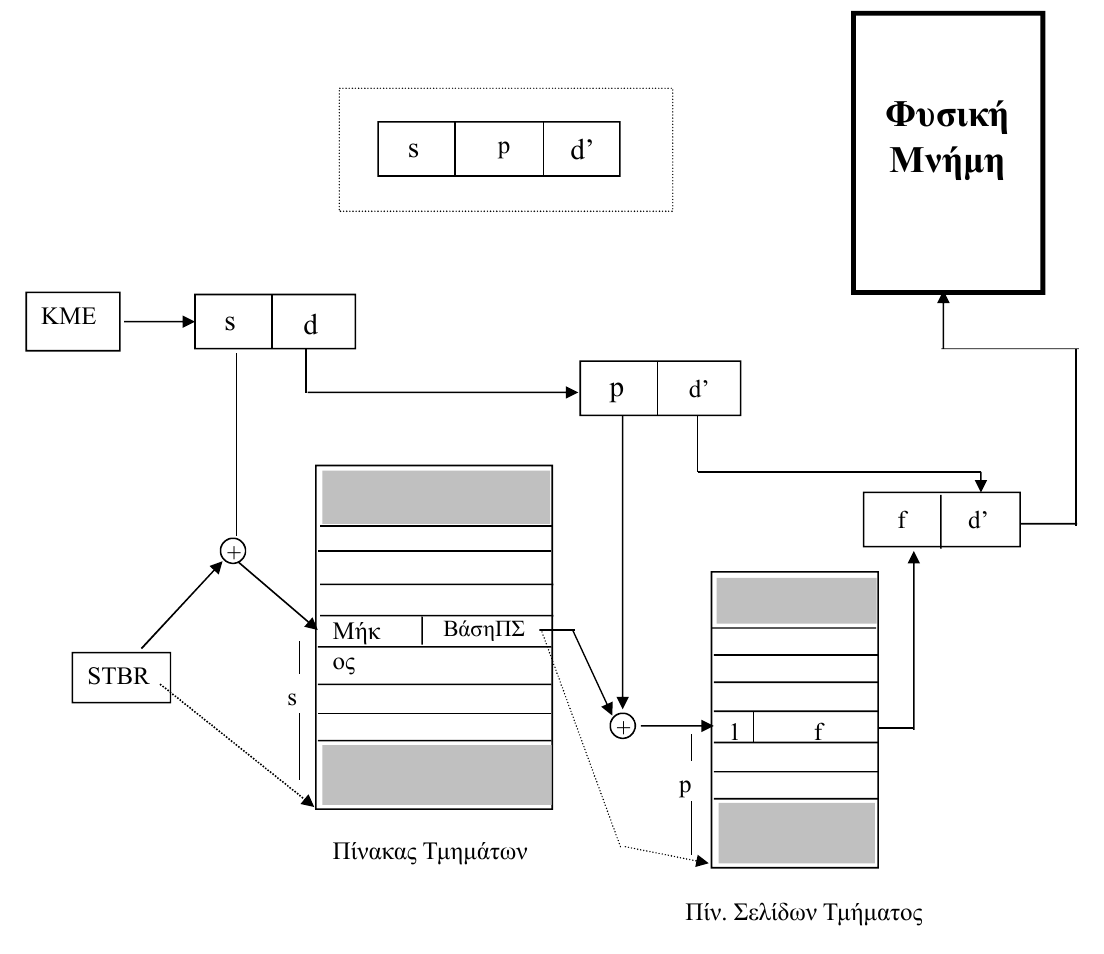
\includegraphics[width=0.75\textwidth]{paged_segmentation.png}
	\caption{Paged Segmentation (για τους όρους βλέπε τμηματοποίηση και σελιδοποίηση)}
\end{figure}

\subsubsection{Τμηματοποιημένη Σελιδοποίηση}

Οταν ο πίνακας σελίδων είναι πολύ μεγάλος...
\begin{itemize}
	\item	Μπορούμε να τον τμηματοποιήσουμε Segmented Paging = τμηματοποίηση του πίνακα σελίδων 
		σε περισσότερα (μεταβλητού μεγέθους) τμήματα.
	\item	Κάθε τμήμα του πίνακα σελίδων μπορούμε να το διαχειριστούμε
		ανεξάρτητα και είτε να βρίσκεται φορτωμένο στη μνήμη είτε όχι
		(ανάλογα με το αν χρησιμοποιείται συχνά από τη διεργασία).
	\item	Μεγάλα τμήματα στο τέλος του Πίνακα Σελίδων που είναι
		άχρηστα μπορούμε να τα διαχειριστούμε αποτελεσματικά χωρίς
		να καταλαμβάνουν χώρο στη μνήμη.
	\item	Καθώς έχουμε πολλαπλά μικρά τμήματα αντί ενός πολύ μεγάλου,
		είναι πιο εύκολη η διαδικασία εύρεσης και εκχώρησης
		ακολουθιακού χώρου μνήμης για κάθε ένα από αυτά
\end{itemize}


\paragraph{Η λογική διεύθυνση U (n bits) τώρα χωρίζεται σε 3 τμήματα.}

\begin{center}
\begin{tabularx}{0.95\textwidth}{|X|X|X|}
\hline
\multicolumn{2}{|l|}{Αριθμός Ιδεατής Σελίδας p(n bits)} & {Μετατόπιση d (k bits)} \\
\hline
Αρ. Τμήματος του Π.Σ. s & Μετατ. στο τμήμα p' & {} \\
\hline
\end{tabularx}
\end{center}

\paragraph{Και μετατρέπεται σε φυσική διεύθυνση Φ στη μορφή:}

\begin{center}
\begin{tabularx}{0.95\textwidth}{XX}
Αριθμός Φυσικής Σελίδας f(m-k' bits) & + Μετατόπιση d' (k' bits)
\end{tabularx}
\end{center}

Οπου m είναι τα bits της Τελικής Φυσικής Διεύθυνσης αν το
συνολικό μέγεθος αυτής θεωρηθεί 
$$ M = 2^m $$

\subsection{Αντικατάσταση σελίδων}
\begin{itemize}
	\item	Προστασία: χρήση ξεχωριστού πίνακα σελίδων για κάθε διεργασία.
	\item	Αλγόριθμοι αντικατάστασης:
		\begin{itemize}
			\item	First-In-First-Out (FIFO)
			\item	Least Recently Used (LRU)
			\item	Longest Residence in Memory (LRM)
			\item	Least Frequently Used (LFU)
		\end{itemize}
\end{itemize}

\subsubsection{FIFO}

Αντικατέστησε την παλαιότερη σελίδα (αυτή που έχει εισαχθεί πρώτη).
Προβλήματα:
\begin{itemize}
	\item	Μπορεί οι παλιές σελίδες να χρησιμοποιούνται συχνά.
	\item	Τα σφάλματα αναφοράς μπορεί να αυξηθούν 
		όσο αυξάνονται τα πλαίσια σελίδας!!! (Belady’s Anomaly)
\end{itemize}

\subsubsection{Αλγόριθμος $2^\text{ης}$ Ευκαιρίας}

\begin{itemize}
	\item	Βασίζεται στη στρατηγική FIFO: εξετάζει σελίδες αρχίζοντας
		από την πιο παλιά αλλά χρησιμοποιεί και bit αναφοράς.
	\item	1η αναφορά σε σελίδα και τοποθέτησή της σε πλαίσιο -> R = 1
	\item	Επιλέγει την πιο παλιά σελίδα και εξετάζει το R bit.
		\begin{itemize}
			\item	Αν R=0 τότε την αντικαθιστά και η νέα σελίδα έχει R = 1.
			\item	Αν R = 1 τότε
				\begin{itemize}
					\item	κάνει το bit R = 0
					\item	η σελίδα τοποθετείται στο τέλος της λίστας 
						(δηλ. "βαφτίζεται" σαν η πιο πρόσφατη σελίδα).
					\item	η αναζήτηση θύματος συνεχίζεται στην επόμενη πιο παλιά σελίδα.
				\end{itemize}
			\item	Αν R=1 για όλες τις σελίδες, τότε second-chance είναι στην ουσία FIFO, 
				γιατί κάνει τα R όλων των σελίδων 0 και μετά επίλέγει την παλιότερη όπως ο FIFO.
		\end{itemize}
\end{itemize}

\subsubsection{LRU}

\begin{itemize}
	\item	Αντικατέστησε τη σελίδα που δεν έχει χρησιμοποιηθεί για το μεγαλύτερο διάστημα.
	\item	Προβλήματα:
		\begin{itemize}
			\item	"Ακριβή" υλοποίηση: π.χ. Ανάγκη διατήρησης χρονικής πληροφορίας
				(time stamp) για κάθε σελίδα.
		\end{itemize}
\end{itemize}
